%% Based on a TeXnicCenter-Template by Tino Weinkauf.
%%%%%%%%%%%%%%%%%%%%%%%%%%%%%%%%%%%%%%%%%%%%%%%%%%%%%%%%%%%%%

%%%%%%%%%%%%%%%%%%%%%%%%%%%%%%%%%%%%%%%%%%%%%%%%%%%%%%%%%%%%%
%% HEADER
%%%%%%%%%%%%%%%%%%%%%%%%%%%%%%%%%%%%%%%%%%%%%%%%%%%%%%%%%%%%%
\documentclass[a4paper,oneside,10pt]{report}
% Alternative Options:
%	Paper Size: a4paper / a5paper / b5paper / letterpaper / legalpaper / executivepaper
% Duplex: oneside / twoside
% Base Font Size: 10pt / 11pt / 12pt


%% Language %%%%%%%%%%%%%%%%%%%%%%%%%%%%%%%%%%%%%%%%%%%%%%%%%
\usepackage[dutch]{babel} %francais, polish, spanish, ...
\usepackage[T1]{fontenc}
\usepackage[ansinew]{inputenc}

\usepackage{lmodern} %Type1-font for non-english texts and characters

%% Packages for Graphics & Figures %%%%%%%%%%%%%%%%%%%%%%%%%%
\usepackage{graphicx} %%For loading graphic files
%\usepackage{subfig} %%Subfigures inside a figure
%\usepackage{tikz} %%Generate vector graphics from within LaTeX

%% Please note:
%% Images can be included using \includegraphics{filename}
%% resp. using the dialog in the Insert menu.
%% 
%% The mode "LaTeX => PDF" allows the following formats:
%%   .jpg  .png  .pdf  .mps
%% 
%% The modes "LaTeX => DVI", "LaTeX => PS" und "LaTeX => PS => PDF"
%% allow the following formats:
%%   .eps  .ps  .bmp  .pict  .pntg


%% Math Packages %%%%%%%%%%%%%%%%%%%%%%%%%%%%%%%%%%%%%%%%%%%%
\usepackage{amsmath}
\usepackage{amsthm}
\usepackage{amsfonts}


%% Line Spacing %%%%%%%%%%%%%%%%%%%%%%%%%%%%%%%%%%%%%%%%%%%%%
%\usepackage{setspace}
%\singlespacing        %% 1-spacing (default)
%\onehalfspacing       %% 1,5-spacing
%\doublespacing        %% 2-spacing


%% Other Packages %%%%%%%%%%%%%%%%%%%%%%%%%%%%%%%%%%%%%%%%%%%
%\usepackage{a4wide} %%Smaller margins = more text per page.
%\usepackage{fancyhdr} %%Fancy headings
%\usepackage{longtable} %%For tables, that exceed one page
\usepackage{algorithm}
\usepackage{algorithmic}
\usepackage{tabularx}
\usepackage{listings}

%%%%%%%%%%%%%%%%%%%%%%%%%%%%%%%%%%%%%%%%%%%%%%%%%%%%%%%%%%%%%
%% Remarks
%%%%%%%%%%%%%%%%%%%%%%%%%%%%%%%%%%%%%%%%%%%%%%%%%%%%%%%%%%%%%
%
% TODO:
% 1. Edit the used packages and their options (see above).
% 2. If you want, add a BibTeX-File to the project
%    (e.g., 'literature.bib').
% 3. Happy TeXing!
%
%%%%%%%%%%%%%%%%%%%%%%%%%%%%%%%%%%%%%%%%%%%%%%%%%%%%%%%%%%%%%

%%%%%%%%%%%%%%%%%%%%%%%%%%%%%%%%%%%%%%%%%%%%%%%%%%%%%%%%%%%%%
%% Options / Modifications
%%%%%%%%%%%%%%%%%%%%%%%%%%%%%%%%%%%%%%%%%%%%%%%%%%%%%%%%%%%%%

%\input{options} %You need a file 'options.tex' for this
%% ==> TeXnicCenter supplies some possible option files
%% ==> with its templates (File | New from Template...).



%%%%%%%%%%%%%%%%%%%%%%%%%%%%%%%%%%%%%%%%%%%%%%%%%%%%%%%%%%%%%
%% DOCUMENT
%%%%%%%%%%%%%%%%%%%%%%%%%%%%%%%%%%%%%%%%%%%%%%%%%%%%%%%%%%%%%
\begin{document}
\pagestyle{empty} %No headings for the first pages.
\floatname{algorithm}{Algoritme} % Geen automatische vertaling van Algorithm -> Algoritme
\renewcommand{\listalgorithmname}{Lijst van algoritmen}

%% Title Page %%%%%%%%%%%%%%%%%%%%%%%%%%%%%%%%%%%%%%%%%%%%%%%
%% ==> Write your text here or include other files.
\begin{titlepage}

\begin{center}

%\vspace*{1cm}
\Large
\textsc{Universiteit van Groningen}\\

\vspace{5cm}

%\LARGE
\textsc{Gevorderde Algoritmen en Datastructuren\\[0.5\baselineskip]
door\\[0.5\baselineskip]
Jos van der Til \& Rene Zuidhof}\\

\vspace{5cm}
\textsc{\today}\\ %%Date - better you write it yourself.

\vspace{1cm}
\end{center}

\end{titlepage}

%% Inhaltsverzeichnis %%%%%%%%%%%%%%%%%%%%%%%%%%%%%%%%%%%%%%%
\tableofcontents %Table of contents
\cleardoublepage %The first chapter should start on an odd page.

\pagestyle{plain} %Now display headings: headings / fancy / ...

%% Chapters %%%%%%%%%%%%%%%%%%%%%%%%%%%%%%%%%%%%%%%%%%%%%%%%%
%% ==> Write your text here or include other files.

%\input{intro} %You need a file 'intro.tex' for this.
\chapter{Introductie}

Dit verslag maakt deel uit van de cursus Gevorderde Algoritmen en Datastructuren van de Rijksuniversiteit Groningen. 
In dit verslag zal de tweede practicum opdracht behandeld worden. 
Deze opdracht omvat het vinden van een maximum flow in een flow network en de verschillende manieren, om dit te doen, te analyseren.

In hoofdstuk \ref{chap:maxFlowProblem} zal het probleem van het vinden van een maximum flow en het gebruikte algoritme beschreven worden. De hoofdstukken \ref{chap:depthfirst}, \ref{chap:breadthfirst} \& \ref{chap:priorityfirst} beschrijven de algoritmen die gebruikt worden om een pad te vinden door het netwerk. De conclusies van dit onderzoek staan in hoofdstuk \ref{chap:conclusion}.

Omdat het Ford-Fulkerson algoritme niet aangeeft op welke manier er een 'augmenting path' gevonden dient te worden, zijn er meerdere methodes beschikbaar.
De methodes die onderzocht zullen worden in dit document zijn:

\begin{enumerate}
	\item Depth-first search;
	\item Breadth-first search;
	\item Priority-first search.
\end{enumerate}

In het geval van een breadth-first search is het algoritme ook bekend als het Edmonds-Karp algoritme.
\chapter{Software}
\label{chap:software}

Om de methodes te visualiseren is een GUI ontwikkeld, deze zal in dit hoofdstuk beschreven worden. In figuur \ref{fig:FFA} is de GUI te zien. De linkerkant laat de graaf zien, en aan de rechterkant zijn controllers aanwezig om de software te bedienen. De start- en eindknoop hebben de kleur groen en rood, respectievelijk. De paden waarover een flow wordt gestuurd zijn blauw gekleurd.

De knop 'Next flow' zal \'e\'en augmented path zoeken met behulp van de methode die gekozen kan worden in de dropdown box. Wanneer een augmented path is gevonden zal de maximale flow voor dat pad er doorheen gestuurd worden. De knop 'Max flow' zal de actie die gedaan wordt voor de knop 'Next flow' uitvoeren tot er geen augmented path meer te vinden is. 

De dropdown box die zojuist genoemd is, is te vinden aan de rechterkant van de knop 'Max flow'. In deze dropdown box kan gekozen worden voor de methode die gebruikt dient te worden voor het zoeken naar een augmented path. Er kan gekozen worden tussen $DFS$ (Depth-first search), $BFS$ (Breadth-first search) en $DIJKSTRA$ (Dijkstra's algorime). 
De knop daarnaast, 'Reset', zal alle waardes voor de graaf weer op hun oorspronkelijke waarde zetten.

Onder de zojuist genoemde knoppen is een knop en een veld te vinden waarmee een graaf bestand geladen kan worden, deze bestanden moeten geplaatst zijn in de hoofdmap van de software. Wanneer een bestandsnaam is ingevoerd en de knop 'Load' wordt ingedrukt zal de graaf geladen worden aan de linkerkant.
Onder de knop 'Load' en het invoerveld is een veld te vinden waarin de status van de graaf en het algoritme weergegeven wordt.

\begin{figure}[h]
	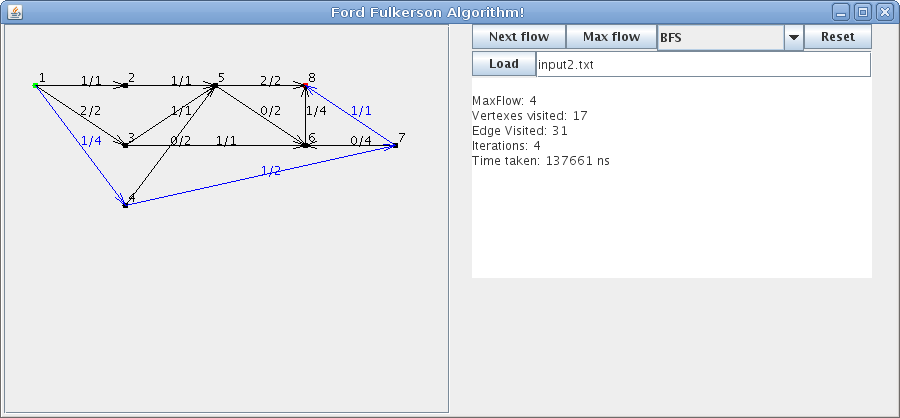
\includegraphics[width=\linewidth]{software/FFA}
	\centering
	\caption{Screenshot van de GUI}
	\label{fig:FFA}
\end{figure}

Hieronder is een voorbeeld te zien van de opbouw van het bestand voor graaf 1. Op de eerste regel staan respectievelijk het aantal knopen en het aantal kanten.
Op de tweede regel staan de getallen die de start- en eindknoop aangeven ($s$ en $t$).
De overige regels bevatten de kanten van de graaf bestaande uit: de beginknoop, de eindknoop en de capaciteit van de kant.
\begin{table}[h]
\begin{lstlisting}
6 8
1 6
1 2 3
1 3 3
2 3 2
2 4 3
2 6 2
3 5 2
5 6 3
4 6 2
\end{lstlisting}
\caption{Inhoud van een graaf bestand (input1.txt)}
\end{table} 
\chapter{Maximum flow probleem}
\label{chap:maxFlowProblem}
Om het probleem van het vinden van een maximum flow te kunnen begrijpen, volgt hier een korte introductie in de grafentheorie.

Een graaf is een verzameling punten (knopen) die verbonden zijn door lijnen (kanten). De kanten van een graaf kunnen een richting en/of een gewicht hebben. Een voorbeeld van een simpele graaf is te zien in figuur \ref{fig:6ngraph}.

\begin{figure}[h]
	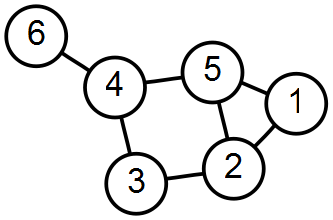
\includegraphics[width=0.5\linewidth]{maxflowproblem/6n-graph}
	\centering
	\caption{Een ongerichte en ongewogen graaf met 6 nodes}
	\label{fig:6ngraph}
\end{figure}

In figuur \ref{fig:flownetwork} is een voorbeeld van een flow network te zien. De flow in deze afbeelding is maximaal, immers de capaciteit van de beide kanten die leiden naar \textit{t} is volledig benut. Tevens te zien dat dit een gerichte (pijlen in plaats van lijnen als kanten) en gewogen (getallen bij de kanten) graaf is.

\begin{figure}[h]
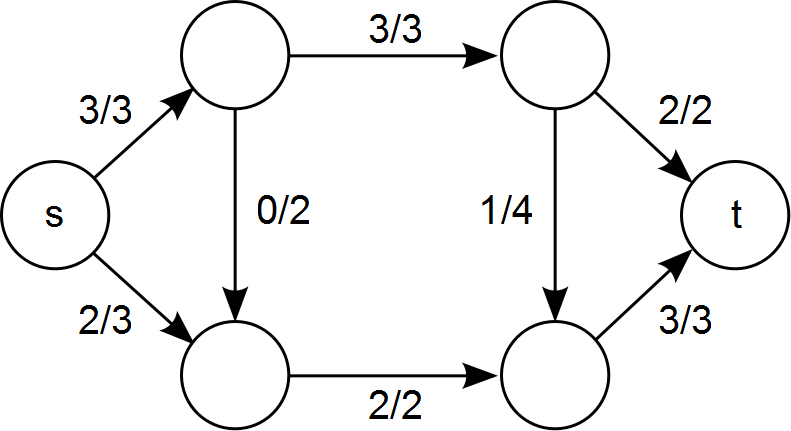
\includegraphics[width=0.5\linewidth]{maxflowproblem/max_flow}%
\centering
\caption{Voorbeeld van een flow netwerk met een maximum flow van \textit{s} naar \textit{t}. De getallen zijn flow / max capaciteit.}%
\label{fig:flownetwork}%
\end{figure}

Het probleem is nu om een flow te vinden van \textit{s} naar \textit{t} die maximaal is. Om dit op te lossen is er het Ford-Fulkerson algoritme, vernoemd naar L.R. Ford en D.R. Fulkerson die dit algoritme publiceerden in 1956. Deze wordt nader toegelicht in paragraaf \ref{sec:fordfulkerson}.

\section{Ford-Fulkerson algoritme}
\label{sec:fordfulkerson}

Het algoritme van Ford \& Fulkerson werkt eigenlijk volgens een heel simpel principe. Zolang er een pad is van \textit{s} naar \textit{t} met beschikbare capaciteit, dan wordt de flow daar langs gestuurd. Dit wordt herhaalt totdat er geen pad meer mogelijk is. Een pad van \textit{s} naar \textit{t} met beschikbare capaciteit wordt een 'augmenting path' genoemd.

De eisen die gesteld worden aan een geldige flow zijn:

\begin{itemize}
	\item De flow mag nooit groter zijn de de capacity van een kant. $0 \leq flow(u,v) \leq capacity(u,v)$
	\item De netto flow van een node is gelijk aan 0. Dit geldt niet voor \textit{s} of \textit{t}.$$\sum_{e \in E^-}\sum_{v \in E^+}{flow(e)-flow(v)} = 0$$
Waar $E^-$ de verzameling van uitgaande kanten is en $E^+$ de verzameling inkomende kanten van knoop $E$ is.
\end{itemize}

Omdat het Ford-Fulkerson algoritme niet aangeeft op welke manier er een 'augmenting path' gevonden dient te worden, zijn er meerdere methodes beschikbaar.
De methodes die onderzocht zullen worden in dit document zijn:

\begin{enumerate}
	\item Depth-first search;
	\item Breadth-first search;
	\item Priority-first search.
\end{enumerate}

\subsection{Pseudocode}

De pseudocode van het Ford-Fulkerson algoritme is te vinden in algoritme \ref{alg:FordFulkerson}.

\begin{algorithm}[h]
\caption{Ford-Fulkerson Algorithm}
\label{alg:FordFulkerson}
\begin{algorithmic}
\REQUIRE Input: Flow network $N$ containing graph $G$
\FORALL{edge $e \in N$}
 \STATE flow($e$) $\gets 0$
\ENDFOR

\STATE $stop \gets$ \FALSE

\REPEAT
\STATE traverse $G$ starting at $s$ to find an augmenting path to $t$ ($\pi$)

\IF{an augmenting path $\pi$ exists}

\STATE $\Delta \gets +\infty$

\FORALL{edge $e \in \pi$}
\IF{ residual capacity($e$) $\leq \Delta$}
\STATE $\Delta \gets $ residual capacity($e$)
\ENDIF
\ENDFOR

\FORALL{edge $e \in \pi$}

\IF{$e$ is a forward edge}
\STATE flow($e$) $\gets $ flow($e$) $+ \Delta$
\ELSE
\STATE flow($e$) $\gets $ flow($e$) $- \Delta$
\ENDIF

\ENDFOR

\ELSE
\STATE $stop \gets$ \TRUE
\ENDIF
\UNTIL{$stop$}

\end{algorithmic}
\end{algorithm}

\section{Analyse}

Voor de analyse van de zoekmethodes worden de grafen uit de figuren \ref{fig:analyseGraaf1} en \ref{fig:analyseGraaf2} gebruikt.
\begin{figure}[h]
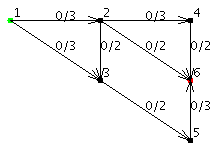
\includegraphics[width=\linewidth]{maxflowproblem/graph1}
\centering
\caption{Analyse graaf 1}
\label{fig:analyseGraaf1}
\end{figure}

\begin{figure}[h]
 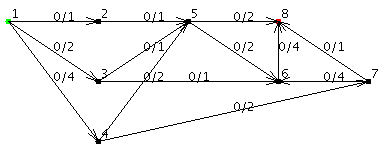
\includegraphics[width=\linewidth]{maxflowproblem/graph2}
\centering
\caption{Analyse graaf 2}
\label{fig:analyseGraaf2}
\end{figure}

\chapter{Depth-first search}
\label{chap:depthfirst}

De eerste methode die onderzocht is voor het zoeken naar een augmented path is de Depth-first search methode. Deze methode zal, zoals de naam suggereert, de diepte in gaan op zoek naar $t$. 


Tijdens het zoeken naar $t$ worden de edges gelabeld met $discovery$, $unexplored$ en $back$. 

\subsection{Pseudocode}
De pseudocode waar de code op gebaseerd is, is te vinden in algoritme \ref{alg:DFS}.

\begin{algorithm}[h]
\caption{Depth-first search Algorithm}
\label{alg:DFS}
\begin{algorithmic}
\REQUIRE Input: Graph g, Start vertex s, End vertex t, HashMap parents with vertexes and its parent edges
\STATE Label s as $EXPLORED$
\FORALL{edge $e \in s.incidentEdges$}
\IF e is not labeled as $UNEXPLORED$ && s.residualCapacity(e) > 0
\STATE w $\gets $ g.opposite(s, e)
\IF w is labeled as $UNEXPLORED$
\STATE label $e$ as $DISCOVERY$ edge
\STATE set $e$ as parent of $w$ in the hashmap parents
\STATE recursive call with g, w, t and parents
\ELSE
\STATE label $e$ as $BACK$ edge
\ENDIF
\ENDIF
\ENDFOR
\end{algorithmic}
\end{algorithm}

Wanneer het eindpunt $t$ bereikt is kan het algoritme stoppen. Nu kan met behulp van de $parents$ gezocht worden naar een pad van $s$ naar $t$ door te kijken wat de parent edge $e$ is van $t$. Nu zal gekeken worden naar de parent edge van de overstaande van $t$ via edge $e$. Door dit te doen tot er geen parent edge is zal $s$ bereikt worden.
\chapter{Breadth-first search}
\label{chap:breadthfirst}

De tweede manier om een augmenting path te vinden in een graaf is de breadth-first search. Deze methode, die ook gebruikt wordt in het Edmonds-Karp algoritme, vindt het kortste pad van $s$ naar $t$. Het kortste pad is in dit geval gedefineert als het pad met het laagste aantal kanten.

Het breadth-first doorlopen van een graaf is niet anders dan dat dat bij een tree gebeurt, elk niveau wordt volledig doorzocht, voordat het algoritme naar het niveau daar onder gaat. Dit is te zien in figuur \ref{fig:breadthFirstTree}, de getallen op de knopen geven aan in welke volgorde de boom doorzocht wordt.

\begin{figure}[h]
 \centering
 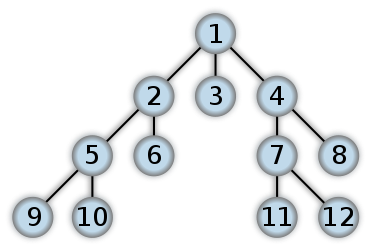
\includegraphics[width=0.5\linewidth]{breadthfirst/breadthfirsttree}
 \label{fig:breadthFirstTree}
 \caption{Breadth-first doorlopen van een boom}
\end{figure}

Om vervolgens het pad van $s$ naar $t$ te vinden in een graaf, wordt eerst de graaf doorlopen volgens het breadth-first principe totdat $t$ gevonden is. Terwijl de graaf doorlopen wordt, wordt bijgehouden welke kant leid naar welke knoop. Hierdoor is het gemakkelijk om het pad van $t$ naar $s$ terug te vinden. De pseudocode voor dit algoritme is te vinden in algoritme \ref{alg:breadthfirst}.

\section{Pseudocode}

\begin{algorithm}
 \caption{Breadth-first search path finding}
 \label{alg:breadthfirst}
 \begin{algorithmic}
  \REQUIRE \textbf{Input}: Graph G, Node s, Node t \\ 
\textbf{Output}: An augmenting path, or an empty path if none found.
  \STATE $Q \gets $ new queue
  \STATE $M \gets $ new hashmap
  \STATE $s$.state $\gets$ \textit{EXPLORED}
  \STATE $Q$.enqueue($s$)
  \WHILE{$\lnot Q$.isEmpty()}
   \STATE $v \gets Q$.dequeue()
   \FORALL{edge $e \in G$.incidentEdges($v$)}
    \IF{$e$.state = \textit{UNEXPLORED} $\land e$.residualCapacity() $ > 0$}
    \STATE $w \gets G$.opposite($v$, $e$)
    \IF{$\lnot w$.state = \textit{EXPLORED}}
      \STATE $Q$.enqueue($w$)
      \STATE $Q$.state = \textit{EXPLORED}
      \STATE $M$.put($w$, $e$) \COMMENT{$w$ discovered through edge $e$}
      \STATE $e$.state = \textit{DISCOVERY}
      \IF{$e$.start = $w$}
         \STATE Mark $e$ as forward
      \ELSE
         \STATE Mark $e$ as backward
      \ENDIF

      \IF{$w = t$}
         \STATE pathFound $\gets \FALSE$
         \STATE $p \gets w$
         \STATE $path \gets $ new list
         \WHILE{$\lnot$pathFound}
          \STATE $c \gets M$.get($p$) \COMMENT{Retreive edge $c$ that led to $p$}
          \STATE $path$.add($c$)      \COMMENT{Add edge $c$ to the path}
          \STATE $p \gets G$.opposite($p$, $c$) \COMMENT{ Go back another step in the graph}
          \IF{$p = s$}
            \STATE pathFound $\gets \TRUE$ \COMMENT{We found the start node, we are done.}
          \ENDIF
         \ENDWHILE
         \RETURN path
      \ENDIF
    \ENDIF
    \ELSE
      \STATE $e$.state $\gets$ \textit{BACKWARD}
    \ENDIF
   \ENDFOR
  \ENDWHILE
  \RETURN empty list \COMMENT{No path found}
 \end{algorithmic}
\end{algorithm}

\section{Analyse}
\chapter{Priority First Search}
\chapter{Conclusie}
\label{chap:conclusion}

%%%%%%%%%%%%%%%%%%%%%%%%%%%%%%%%%%%%%%%%%%%%%%%%%%%%%%%%%%%%%
%% BIBLIOGRAPHY AND OTHER LISTS
%%%%%%%%%%%%%%%%%%%%%%%%%%%%%%%%%%%%%%%%%%%%%%%%%%%%%%%%%%%%%
%% A small distance to the other stuff in the table of contents (toc)
\addtocontents{toc}{\protect\vspace*{\baselineskip}}

%% The List of Figures
\clearpage
\addcontentsline{toc}{chapter}{Lijst van figuren}
\listoffigures

%% The List of Tables
\clearpage
\addcontentsline{toc}{chapter}{Lijst van tabellen}
\listoftables

\clearpage
\addcontentsline{toc}{chapter}{\listalgorithmname}
\listofalgorithms


%%%%%%%%%%%%%%%%%%%%%%%%%%%%%%%%%%%%%%%%%%%%%%%%%%%%%%%%%%%%%
%% APPENDICES
%%%%%%%%%%%%%%%%%%%%%%%%%%%%%%%%%%%%%%%%%%%%%%%%%%%%%%%%%%%%%
\appendix
%\input{FileName} %You need a file 'FileName.tex' for this.
\chapter{Source Code}
\chapter{AugmentedPath}
\lstset{language=Java}
\begin{lstlisting}[caption=AugmentedPath Source Code]
public abstract class AugmentedPath {

	public enum Method {DFS, BFS, DIJKSTRA}
	
	protected static Profiler profiler = new Profiler();
	
	public static final AugmentedPath NULL = new NullPath();
	
	public abstract List<Edge> getAugmentedPath(Graph g, Vertex s, Vertex t);
	
	protected static List<Edge> findAugmentedPath(HashMap<Vertex, Edge> parents, Graph g, Vertex s, Vertex t){
		List<Edge> augmentedPath = new LinkedList<Edge>();
		Vertex iterator = t;
		Edge parent = parents.get(iterator);
		boolean sourceReached = false;
		while(parent != null){
			augmentedPath.add(parent);
			iterator = g.opposite(iterator, parent);
			parent = parents.get(iterator);
			if(iterator.equals(s)){
				sourceReached = true;
			}
		}
		if(sourceReached){
			return augmentedPath;
		}
		return Collections.emptyList();
	}

	public static Profiler getProfiler() {
		return profiler;
	}

	private static final class NullPath extends AugmentedPath {
		@Override
		public List<Edge> getAugmentedPath(Graph g, Vertex s, Vertex t) {
			return Collections.emptyList();
		}
	}
	
}
\end{lstlisting}
\chapter{AugmentedPathBFS}
\lstset{language=Java}
\begin{lstlisting}[caption=AugmentedPathBFS Source Code]
ublic class AugmentedPathBFS extends AugmentedPath {

	public List<Edge> getAugmentedPath(Graph g, Vertex s, Vertex t) {
		List<Edge> path = new LinkedList<Edge>();
		Queue<Vertex> vertexQueue = new LinkedList<Vertex>();
		
		//Map <x,y>. Vertex y discovered by following x
		Map<Vertex, Edge> discoveryMap = new HashMap<Vertex, Edge>(); 

		s.status = VertexStatus.EXPLORED;
		vertexQueue.add(s);

		Vertex w;
		List<Edge> unionEdge;

		while (!vertexQueue.isEmpty()) {
			w = vertexQueue.poll();
			profiler.visitedVertex();
			unionEdge = w.getAllEdges();
			for (Edge e : unionEdge) {
				if (e.status == EdgeStatus.UNEXPLORED
						&& (w.getResidualCapacity(e) > 0)) {
					profiler.visitedEdge();
					Vertex next = g.opposite(w, e);
					if (next.status == VertexStatus.UNEXPLORED) {
						vertexQueue.add(next);
						discoveryMap.put(next, e);
						next.status = VertexStatus.EXPLORED;
						e.status = EdgeStatus.DISCOVERY;
						
						if (e.start.equals(w)) {
							e.forward = true;
						} else {
							e.forward = false;
						}
						
						if (next == t) {
							//sink found. Trace back.
							boolean traceDone = false;
							Edge currentEdge;
							Vertex previousVertex = next;
							while(!traceDone) {
								currentEdge = discoveryMap.get(previousVertex);
								path.add(currentEdge);
								
								previousVertex = g.opposite(previousVertex, currentEdge);
								
								if(previousVertex == s)
									traceDone = true;
							}
							
							return path;
						}
					} else {
						e.status = EdgeStatus.BACK;
					}
				}
			}

			unionEdge = null;
		}

		return path;
	}
	
}
\end{lstlisting}
\chapter{AugmentedPathDFS}
\lstset{language=Java}
\begin{lstlisting}[caption=AugmentedPathDFS Source Code]
public class AugmentedPathDFS extends AugmentedPath {

	private boolean stop = false;
	
	public List<Edge> getAugmentedPath(Graph g, Vertex s, Vertex t){
		HashMap<Vertex, Edge> parents = getPathDFS(g, s, t, new HashMap<Vertex, Edge>());
		return findAugmentedPath(parents, g, s, t);
	}
	
	public HashMap<Vertex, Edge> getPathDFS(Graph g, Vertex s, Vertex t, HashMap<Vertex, Edge> parents) {
		s.status = VertexStatus.EXPLORED;
		profiler.visitedVertex();
		stop = false;
		for (Edge e : s.getAllEdges()) {
			if (e.status == EdgeStatus.UNEXPLORED
					&& s.getResidualCapacity(e) > 0) {
				profiler.visitedEdge();
				Vertex w = g.opposite(s, e);
				if (w.status == VertexStatus.UNEXPLORED) {
					e.status = EdgeStatus.DISCOVERY;
					//profiler.visitedVertex();
					parents.put(w, e);
					if (e.start.equals(s)) {
						e.forward = true;
					} else {
						e.forward = false;
					}
					if(w.equals(t)){
						stop = true;
						return parents;
					}
					getPathDFS(g, w, t, parents);
				} else {
					e.status = EdgeStatus.BACK;
				}
			}
			if(stop){
				return parents;
			}
		}
		return parents;
	}
}
\end{lstlisting}
\chapter{AugmentedPathDijkstra}
\lstset{language=Java}
\begin{lstlisting}[caption=AugmentedPathDijkstra Source Code]
public class AugmentedPathDijkstra extends AugmentedPath {

	public List<Edge> getAugmentedPath(Graph g, Vertex s, Vertex t){
		HashMap<Vertex, Edge> parents = new HashMap<Vertex, Edge>();
		PriorityQueue<Vertex> Q = new PriorityQueue<Vertex>();
		for(Vertex v : g.vertexList){
			if(v.equals(s)){
				v.maxFlow = Integer.MAX_VALUE;
			} else {
				v.maxFlow = 0;
			}
			Q.add(v);
			parents.put(v, null);
		}
		while(!Q.isEmpty()){
			Vertex u = Q.remove();
			profiler.visitedVertex();
			if(u.equals(t)){
				return findAugmentedPath(parents, g, s, t);
			}
			for(Edge e : u.getAllEdges()){
				profiler.visitedEdge();
				Vertex z = g.opposite(u, e);
				int r = Math.min(u.getResidualCapacity(e), u.maxFlow);
				if(r > z.maxFlow && !e.equals(parents.get(z))){
					z.maxFlow = r;
					parents.put(z, e);
					if (e.start.equals(u)) {
						e.forward = true;
					} else {
						e.forward = false;
					}
					if(Q.remove(z)){
						Q.add(z);
					}
				}
			}
		}
		return Collections.emptyList();
	}
	
}
\end{lstlisting}
\chapter{Controller}
\lstset{language=Java}
\begin{lstlisting}[caption=Controller Source Code]
public class Controller {

	private View view;
	private MaxFlowFordFulkerson mfff;
	
	public Controller(){
		view = new View();
		view.addNextFlowListener(nextFlowListener());
		view.addFindMaxFlowListener(findMaxFlowListener());
		view.addResetListener(resetListener());
		view.addLoadListener(loadFileListener());
	}
	
	private void loadGraphFile(String fileName){
		File file = new File(fileName);
		if(!file.exists()){
			JOptionPane.showMessageDialog(new JFrame(),
				    "File not found!",
				    "Warning!",
				    JOptionPane.WARNING_MESSAGE);
			return;
		}
		Graph graph = GraphBuilder.buildGraph(file);
		mfff = new MaxFlowFordFulkerson(graph, graph.startPoint, graph.endPoint);
		mfff.setGraphListener(updateViewListener());
		mfff.completeReset();
		view.loadGraph(graph);
	}
	
	private ActionListener loadFileListener(){
		return new ActionListener() {
			@Override
			public void actionPerformed(ActionEvent e) {
				loadGraphFile(view.getFileName());
			}
		};
	}
	
	private ActionListener findMaxFlowListener(){
		return new ActionListener() {
			@Override
			public void actionPerformed(ActionEvent e) {
				if(mfff == null){
					JOptionPane.showMessageDialog(new JFrame(),
						    "No graph loaded yet!",
						    "Warning!",
						    JOptionPane.WARNING_MESSAGE);
					return;
				}
				mfff.findMaxFlow(view.getSelectedMethod());
			}
		};
	}
	
	private ActionListener nextFlowListener(){
		return new ActionListener() {
			@Override
			public void actionPerformed(ActionEvent e) {
				if(mfff == null){
					JOptionPane.showMessageDialog(new JFrame(),
						    "No graph loaded yet!",
						    "Warning!",
						    JOptionPane.WARNING_MESSAGE);
					return;
				}
				mfff.nextFlow(view.getSelectedMethod());
			}
		};
	}
	
	private ActionListener resetListener(){
		return new ActionListener() {
			@Override
			public void actionPerformed(ActionEvent e) {
				if(mfff == null){
					JOptionPane.showMessageDialog(new JFrame(),
						    "No graph loaded yet!",
						    "Warning!",
						    JOptionPane.WARNING_MESSAGE);
					return;
				}
				mfff.completeReset();
			}
		};
	}
	
	private ActionListener updateViewListener(){
		return new ActionListener() {
			@Override
			public void actionPerformed(ActionEvent e) {
				view.updateGraph();
				view.setLabelText(e.getActionCommand());
			}
		};
	}
	
	public static void main(String args[]){
		new Controller();
	}
}
\end{lstlisting}
\chapter{Controllers}
\lstset{language=Java}
\begin{lstlisting}[caption=Controllers Source Code]
public class Controllers extends JPanel {

	private static final long serialVersionUID = 2396396168572312934L;
	private JButton nextFlowButton = new JButton("Next flow");
	private JButton findMaxFlowButton = new JButton("Max flow");
	private JComboBox methodBox;
	private JButton resetButton = new JButton("Reset");
	private JTextArea label = new JTextArea("");
	private JButton loadButton = new JButton("Load");
	private JTextField inputFileField = new JTextField("input1.txt");
	
	private Box topBox = Box.createHorizontalBox();
	private Box middleBox = Box.createHorizontalBox();
	private Box bottomBox = Box.createHorizontalBox();
	
	public Controllers(){
		setLayout(new BoxLayout(this, BoxLayout.Y_AXIS));
		
		Dimension d = new Dimension(400, 27);
		topBox.setMaximumSize(d);
		middleBox.setMaximumSize(d);
		
		Dimension d2 = new Dimension(400, 200);
		bottomBox.setMaximumSize(d2);
		add(topBox);
		add(middleBox);
		add(bottomBox);
		
		topBox.add(nextFlowButton);
		methodBox = new JComboBox();
		methodBox.addItem(Method.DFS);
		methodBox.addItem(Method.BFS);
		methodBox.addItem(Method.DIJKSTRA);
		topBox.add(findMaxFlowButton);
		topBox.add(methodBox);
		topBox.add(resetButton);
		
		middleBox.add(loadButton);
		
		middleBox.add(inputFileField);
		
		label.setEditable(false);
		bottomBox.add(label);

	}
	
	public void addFindMaxFlowListener(ActionListener al){
		findMaxFlowButton.addActionListener(al);
	}
	
	public void addResetListener(ActionListener al){
		resetButton.addActionListener(al);
	}
	
	public String getFileName(){
		return inputFileField.getText();
	}
	
	public void addLoadListener(ActionListener al){
		loadButton.addActionListener(al);
	}
	
	public void addNextFlowButtonListener(ActionListener al){
		nextFlowButton.addActionListener(al);
	}
	
	public Method getSelectedMethod(){
		return (Method) methodBox.getSelectedItem();
	}
	
	public void setLabelText(String text){
		label.setText(text);
	}
}
\end{lstlisting}
\chapter{Edge}
\lstset{language=Java}
\begin{lstlisting}[caption=Edge Source Code]
public class Edge {

	public final int capacity;
	public int flow;
	public Vertex start;
	public Vertex end;
	public Color color = Color.black;
	
	//To be used when on the search for an augmenting path
	//Not to be used when creating a graph
	public boolean forward = true;
	
	public enum EdgeStatus {UNEXPLORED, BACK, DISCOVERY};
	public EdgeStatus status = EdgeStatus.UNEXPLORED;
	
	public Edge(int capacity) {
		this.capacity = capacity;
	}
}
\end{lstlisting}
\chapter{Graph}
\lstset{language=Java}
\begin{lstlisting}[caption=Graph Source Code]
public class Graph {
	
	public List<Edge> edgeList;
	public List<Vertex> vertexList;
	
	public Vertex startPoint;
	public Vertex endPoint;
	
	public void setStartPoint(Vertex v) {
		edgeList = new LinkedList<Edge>();
		vertexList = new LinkedList<Vertex>();
		this.startPoint = v;
		insert(v);
	}
	
	public void setEndPoint(Vertex v) {
		this.endPoint = v;
		insert(v);
	}
	
	public Vertex opposite(Vertex v, Edge e){
		if(e.start.equals(v)){
			return e.end;
		}
		return e.start;
	}
	
	//insert(Vertex)
	public void insert(Vertex v) {
		this.vertexList.add(v);
	}
	
	//insert(Edge e, Vertex start, Vertex eind)
	public void insert(Edge e, Vertex start, Vertex end) {
		edgeList.add(e);
		e.start = start;
		e.end = end;
		start.addOutgoing(e);
		end.addIncoming(e);
	}
	
	//areAdjacent(Vertex a, Vertex b)
	public boolean areAdjacent(Vertex a, Vertex b) {
		for(Edge e : a.outgoingEdges) {
			if(e.end == b)
				return true;
		}
		
		return false;
	}
	
	public Edge getConnectingEdge(Vertex a, Vertex b) {
		for(Edge e : a.outgoingEdges) {
			if(e.end == b)
				return e;
		}
		
		return null;
	}
	
	/**
	 * Finds a Vertex with the specified id within the vertexList.
	 * 
	 * Access time O(n). Where n is the number of vertexes
	 * 
	 * @param id
	 * @return The vertex, or null.
	 */
	public Vertex findVertex(int id) {
		for(Vertex v : vertexList)
			if(v.id == id)
				return v;
		
		return null;
	}
	
	public void printGraph(){
		for(Vertex v : this.vertexList){
			System.out.println("Vertex " + v.id);
			for(Edge e : v.outgoingEdges){
				System.out.println("ForwardEdge to " + e.end.id + " Flow: " + e.flow + "/" + e.capacity);
			}
			for(Edge e : v.incomingEdges){
				System.out.println("BackwardEdge to " + e.start.id + " Flow: " + e.flow + "/" + e.capacity);
			}
		}
	}
\end{lstlisting}
\chapter{GraphBuiler}
\lstset{language=Java}
\begin{lstlisting}[caption=GraphBuiler Source Code]
public class GraphBuilder {

	public static Graph buildGraph(File f) {
		BufferedReader reader = null;
		Graph g = new Graph();
		
		try {
			reader = new BufferedReader(new FileReader(f));
			
			String line = reader.readLine();
			
			String[] split = line.split(" ");
			int numVertexes = Integer.parseInt(split[0]);
			int numEdges = Integer.parseInt(split[1]);
			
			line = reader.readLine();
			split = line.split(" ");
			
			int start = Integer.parseInt(split[0]);
			int end = Integer.parseInt(split[1]);
			
			
			Vertex a = new Vertex(start);
			Vertex b = new Vertex(end);
					
			g.setStartPoint(a);
			g.setEndPoint(b);
			
			for(int m = 0; m < numEdges; ++m) {
				line = reader.readLine();
				
				if(line == null) {
					throw new IOException("Unexpected end of edge list.");
				}
				
				split = line.split(" ");
				
				if(split.length != 3) {
					throw new IOException("Malformed input: " + line);
				}
				
				int s = Integer.parseInt(split[0]); //Start vertex
				int e = Integer.parseInt(split[1]); //End vertex
				int c = Integer.parseInt(split[2]); //Capacity
				
				a = g.findVertex(s);
				b = g.findVertex(e);
				
				if(a == null) {
					a = new Vertex(s);
					g.insert(a);
				}
				
				if(b == null) {
					b = new Vertex(e);
					g.insert(b);
				}
				
				g.insert(new Edge(c), a, b);
			}
			
			if(g.vertexList.size() != numVertexes)
				throw new IOException(String.format("Not all vertexes are used? %d declared. %d added", numVertexes, g.vertexList.size()));
			
			
			return g;
		} catch(FileNotFoundException fnfe) {
			System.err.println("File not found: " + f);
		} catch(IOException ioe) {
			ioe.printStackTrace();
		} finally {
			try {
				reader.close();
			}catch(Exception e){}
		}
		
		return null; //Failure, return null! BAM
	}
}
\end{lstlisting}
\chapter{GraphView}
\lstset{language=Java}
\begin{lstlisting}[caption=GraphView Source Code]
public class GraphView extends JPanel {
	
	private static final long serialVersionUID = -8380122751232428458L;
	private Graph graph;
	private HashMap<Vertex, Point> vertexPoints = new HashMap<Vertex, Point>();
	private HashMap<Integer, Integer> xymap = new HashMap<Integer, Integer>();
	private List<Vertex> drawn = new LinkedList<Vertex>();
	
	private int scale = 3;
	
	public GraphView(){
		
	}
	
	public void setGraph(Graph g){
		this.graph = g;
		updateGraph();
	}
	
	public void paint(Graphics g){
		Graphics2D g2 = (Graphics2D)g;
		g2.clearRect(0, 0, this.getWidth(), this.getHeight());
		if(graph == null){
			return;
		}
		vertexPoints.clear();
		drawn.clear();
		xymap.clear();
		draw(graph.startPoint, new Point(10, 20), g2);
	}
	
	private void draw(Vertex v, Point p, Graphics2D g){
		if(!vertexPoints.containsKey(v)){
			vertexPoints.put(v, p);
		}
		p = vertexPoints.get(v);
		drawVertex(v, p, g);
		drawn.add(v);
		
		if(!xymap.containsKey(p.x)){
			xymap.put(p.x, p.y);
		}
		int y = xymap.get(p.x);
		
		for(Edge e : v.getAllEdges()){
			Vertex opposite = graph.opposite(v, e);
			Point p1 = new Point();
			Point p2 = new Point();
			if(vertexPoints.containsKey(opposite)){
				if(e.start.equals(v)){
					p1 = p;
					p2 = vertexPoints.get(opposite);
				} else {
					p1 = vertexPoints.get(opposite);
					p2 = p;
				}
			} else {
				p2 = new Point(p.x + 30, y);
				drawVertex(opposite, p2, g);
				vertexPoints.put(opposite, p2);
				if(e.start.equals(v)){
					p1 = p;
				} else {
					p1 = p2;
					p2 = p;
				}
				y = y + 20;
			}
			drawEdge(e, p1, p2, g);
		}
		
		xymap.put(p.x, y);
		
		for(Edge e : v.getAllEdges()){
			Vertex opposite = graph.opposite(v, e);
			if(!drawn.contains(opposite)){
				Point p2 = vertexPoints.get(opposite);
				draw(opposite, p2, g);
			}
		}
	}
	
	private void drawVertex(Vertex v, Point p, Graphics2D g){
		if(v.equals(graph.startPoint)){
			g.setColor(Color.GREEN);
		} else if(v.equals(graph.endPoint)) {
			g.setColor(Color.red);
		}
		p = new Point(p.x * scale, p.y * scale);
		g.fillOval(p.x - (1 * scale), p.y - (1 * scale), 2 * scale, 2 * scale);
		g.setColor(Color.black);
		g.drawString(v.id + "", p.x + scale, p.y - scale);
		updateSize(p, g);
	}
	
	private void drawEdge(Edge e, Point p1, Point p2, Graphics2D g){
		p1 = new Point(p1.x * scale, p1.y * scale);
		p2 = new Point(p2.x * scale, p2.y * scale);
		
		g.setColor(e.color);
		g.drawLine(p1.x, p1.y, p2.x, p2.y);
		
		double arrowLength = 4 * scale;
		double arrowAngle = 15;
		double angle;
		if(p1.y == p2.y){
			if(p1.x < p2.x){
				angle = 0;
			} else {
				angle = 180;
			}
		} else if(p1.x == p2.x){
			if(p1.y < p2.y){
				angle = 90;
			} else {
				angle = 270;
			}
		} else {
			double xDistance = Math.abs(p2.x-p1.x);
			double yDistance = Math.abs(p2.y-p1.y);
			double xyDistance = Math.sqrt(xDistance*xDistance + yDistance*yDistance);
			angle = Math.toDegrees(Math.acos(xDistance/xyDistance));
			if(p2.y < p1.y){
				angle = 360 - angle;
			}
			if(p2.x < p1.x){
				angle = 180 - angle;
			}
		}
		double y1 = Math.sin(Math.toRadians((angle + arrowAngle))) * arrowLength;
		double x1 = Math.cos(Math.toRadians((angle + arrowAngle))) * arrowLength;
		
		double y2 = Math.sin(Math.toRadians((-angle + arrowAngle))) * arrowLength;
		double x2 = Math.cos(Math.toRadians((-angle + arrowAngle))) * arrowLength;
		
		g.drawLine(p2.x, p2.y, (int)(p2.x - x1), (int)(p2.y - y1));
		g.drawLine(p2.x, p2.y, (int)(p2.x - x2), (int)(p2.y + y2));
		
		g.drawString(e.flow + "/" + e.capacity, (p1.x + p2.x) / 2, (p1.y + p2.y) / 2);
		g.setColor(Color.black);
	}
	
	private void updateSize(Point p, Graphics g){
		Dimension d = new Dimension(getPreferredSize().width, getPreferredSize().height);
		if(p.x > d.width){
			d.width = p.x + 30;
		}
		if(p.y > d.height){
			d.height = p.y + 30;		
		}
		setPreferredSize(d);
		setMaximumSize(d);
		setMinimumSize(d);
		setSize(d);
	}
	
	public void updateGraph(){
		this.repaint();
	}
}
\end{lstlisting}
\chapter{MaxFlowFordFulkerson}
\lstset{language=Java}
\begin{lstlisting}[caption=MaxFlowFordFulkerson Source Code]
public class MaxFlowFordFulkerson {
	
	private Graph g;
	private Vertex s, t;
	
	private ActionListener listener;
	
	//MaxFlowFordFulkerson algorithm described on page 390
	public MaxFlowFordFulkerson(Graph g, Vertex s, Vertex t){
		this.g = g;
		this.s = s;
		this.t = t;
		for(Edge e : g.edgeList){
			e.flow = 0;
		}
	}
	
	public void findMaxFlow(Method m){
		while(!AugmentedPath.getProfiler().getMaxFlowFound()){
			nextFlow(m);
		}
	}
	
	public void nextFlow(Method m){		
		//Reset all directions in graph
		resetGraphStatus();
		AugmentedPath.getProfiler().incIterations();
		AugmentedPath.getProfiler().startStopwatch();
		List<Edge> augmentedPath = getAugmentedPath(m);
		if(augmentedPath.size() > 0){
			int resCap = getResidualCapacity(augmentedPath);
			pushResCap(augmentedPath, resCap);
		} else {
			AugmentedPath.getProfiler().setMaxFlowFound(true);
		}
		AugmentedPath.getProfiler().pauseStopwatch();
		graphChanged(); //Update View
	}
	
	public void completeReset(){
		for(Edge e : g.edgeList){
			e.status = EdgeStatus.UNEXPLORED;
			e.color = Color.black;
			e.flow = 0;
		}
		for(Vertex v : g.vertexList){
			v.status = VertexStatus.UNEXPLORED;
			v.maxFlow = 0;
		}
		AugmentedPath.getProfiler().reset();
		graphChanged(); //Update view
	}
	
	public void resetGraphStatus(){
		for(Edge e : g.edgeList){
			e.status = EdgeStatus.UNEXPLORED;
			e.color = Color.black;
		}
		for(Vertex v : g.vertexList){
			v.status = VertexStatus.UNEXPLORED;
		}
	}
	
	private List<Edge> getAugmentedPath(Method m){
		AugmentedPath ap;
		switch (m) {
		case DFS:
			ap = new AugmentedPathDFS();
			break;
		case BFS:
			ap = new AugmentedPathBFS();
			break;
		case DIJKSTRA:
			ap = new AugmentedPathDijkstra();
			break;
		default:
			ap = AugmentedPath.NULL;
			break;
		}
		return ap.getAugmentedPath(g, s, t);
	}
	
	//Computes the residual capacity of the augmenting path
	private int getResidualCapacity(List<Edge> augmentingPath){
		int maxFlow = Integer.MAX_VALUE;
		for(Edge e : augmentingPath){
			int resCap;
			if(e.forward){
				resCap = e.capacity - e.flow;
			} else {
				resCap = e.flow;
			}
			if(resCap < maxFlow){
				maxFlow = resCap;
			}
		}
		return maxFlow;
	}
	
	//Pushes the residual capacity along the augmenting path
	private void pushResCap(List<Edge> augmentedPath, int resCap){
		for(Edge e : augmentedPath){
			e.color = Color.blue;
			if(e.forward){
				e.flow = e.flow + resCap;
			} else {
				e.flow = e.flow - resCap;
			}
		}
	}
	
	private void graphChanged(){
		AugmentedPath.getProfiler().update(g);
		ActionEvent ae = new ActionEvent(g.startPoint, g.startPoint.id, AugmentedPath.getProfiler().getStatus());
		listener.actionPerformed(ae);
	}
	
	public void setGraphListener(ActionListener listener){
		this.listener = listener;
	}
	
}
\end{lstlisting}
\chapter{Profiler}
\lstset{language=Java}
\begin{lstlisting}[caption=Profiler Source Code]
public class Profiler {

	private int maxFlow;
	private boolean maxFlowFound;
	private int visitedVertexes;
	private int visitedEdges;
	private long totalTime;
	private int iterations;
	
	private long currentTime;
	
	public void reset(){
		maxFlow = 0;
		maxFlowFound = false;
		visitedVertexes = 0;
		visitedEdges = 0;
		totalTime = 0;
		currentTime = 0;
		iterations = 0;
	}
	
	public void startStopwatch(){
		currentTime = System.nanoTime();
	}
	
	public void pauseStopwatch(){
		if(!maxFlowFound){
			totalTime += System.nanoTime() - currentTime;
		}
	}
	
	public void update(Graph g){
		maxFlow = 0;
		for(Edge e : g.startPoint.outgoingEdges){
			maxFlow += e.flow;
		}
		for(Edge e : g.startPoint.incomingEdges){
			maxFlow += e.capacity - e.flow;
		}
	}
	
	public void visitedVertex(){
		if(!maxFlowFound){
			visitedVertexes++;
		}
	}
	
	public void visitedEdge(){
		if(!maxFlowFound){
			visitedEdges++;
		}
	}
	
	public void incIterations(){
		if(!maxFlowFound){
			iterations++;
		}
	}
	
	public void setMaxFlowFound(boolean value){
		maxFlowFound = value;
	}
	
	public boolean getMaxFlowFound(){
		return maxFlowFound;
	}
	
	public String getStatus(){
		String message = "";
		if(maxFlowFound){
			message += "Done!";
		}
		
		message += " \nMaxFlow: " + maxFlow;
		message += " \nVertexes visited: " + visitedVertexes;
		message += " \nEdge Visited: " + visitedEdges;
		message += " \nIterations: " + iterations;
		message += " \nTime taken: " + totalTime + " ns";
				
		return message;
	}
}
\end{lstlisting}
\chapter{Vertex}
\lstset{language=Java}
\begin{lstlisting}[caption=Vertex Source Code]
public class Vertex implements Comparable<Vertex> {
	
	public int id;
	public List<Edge> incomingEdges;
	public List<Edge> outgoingEdges;
	
	//Only used for Dijkstra's algorithm
	public Integer maxFlow = 0;
	
	//Only to be used when searching for augmented path
	public enum VertexStatus {UNEXPLORED, EXPLORED};
	public VertexStatus status = VertexStatus.UNEXPLORED;
	
	public Vertex(int id) {
		this.id = id;
		incomingEdges = new LinkedList<Edge>();
		outgoingEdges = new LinkedList<Edge>();
	}
	
	public void addIncoming(Edge e) {
		incomingEdges.add(e);
	}
	
	public void addOutgoing(Edge e) {
		outgoingEdges.add(e);
	}
	
	public int getResidualCapacity(Edge e){
		if (e.start.equals(this)) {
			return e.capacity - e.flow;
		} else {
			return e.flow;
		}
	}
	
	public List<Edge> getAllEdges(){
		List<Edge> unionEdge = new LinkedList<Edge>();
		unionEdge.addAll(this.incomingEdges);
		unionEdge.addAll(this.outgoingEdges);
		return unionEdge;
	}
	
	@Override
	public int compareTo(Vertex v) {
		return -this.maxFlow.compareTo(v.maxFlow);
	}
}
\end{lstlisting}
\chapter{View}
\lstset{language=Java}
\begin{lstlisting}[caption=View Source Code]
public class View extends JFrame {

	private static final long serialVersionUID = -5640918753333009588L;
	
	private GraphView graphView;
	private Controllers controllers;
	
	public View(){
		super("Ford Fulkerson Algorithm!");
		setLayout(new GridLayout());
		
		graphView = new GraphView();
		controllers = new Controllers();
		
		JScrollPane scrollPane = new JScrollPane(graphView);
		//scrollPane.setHorizontalScrollBarPolicy(JScrollPane.HORIZONTAL_SCROLLBAR_ALWAYS);
		//scrollPane.setVerticalScrollBarPolicy(JScrollPane.VERTICAL_SCROLLBAR_ALWAYS);
		Dimension d = new Dimension(400, 400);
		scrollPane.setPreferredSize(d);
		scrollPane.setMaximumSize(d);
		scrollPane.setMinimumSize(d);
		add(scrollPane);
		
		d.width = 100;
		controllers.setPreferredSize(d);
		controllers.setMaximumSize(d);
		controllers.setMinimumSize(d);
		add(controllers);
		
		setSize(700, 400);
		setDefaultCloseOperation(EXIT_ON_CLOSE);
		setVisible(true);
	}
	
	public void loadGraph(Graph g){
		graphView.setGraph(g);
	}
	
	public void setLabelText(String text){
		controllers.setLabelText(text);
	}
	
	public void addResetListener(ActionListener al){
		controllers.addResetListener(al);
	}
	
	public void addNextFlowListener(ActionListener al){
		controllers.addNextFlowButtonListener(al);
	}
	
	public void addFindMaxFlowListener(ActionListener al){
		controllers.addFindMaxFlowListener(al);
	}
	
	public Method getSelectedMethod(){
		return controllers.getSelectedMethod();
	}
	
	public void addLoadListener(ActionListener al){
		controllers.addLoadListener(al);
	}
	
	public String getFileName(){
		return controllers.getFileName();
	}
	
	public void updateGraph(){
		graphView.updateGraph();
	}
}
\end{lstlisting}
\end{document}

